% Preamble
% ---
\documentclass{article}

% Packages
% ---
\usepackage{amsmath} % Advanced math typesetting
\usepackage[utf8]{inputenc} % Unicode support (Umlauts etc.)
\usepackage[english, ngerman]{babel} % Change hyphenation rules
\usepackage{hyperref} % Add a link to your document
\usepackage{graphicx} % Add pictures to your document
\usepackage{listings} % Source code formatting and highlighting
\usepackage{csquotes}

\usepackage[backend=bibtex,style=verbose-trad2]{biblatex} % Use biblatex package
%\bibliography{quick} % The name of the .bib file (name without .bib)

% Main document
% ---
\begin{document}
\selectlanguage{english}
% Set up the maketitle command
\author{Georges Leschener M. Essomba}
\title{PhD Research Project Overview}
\date{18th January 2019}

\maketitle{} % Generates title

\pagebreak % Start new page.
\tableofcontents % Generates table of contents from sections

\pagebreak % Start new page
\section{Project overview}


Microservices are gaining more and more popularity as the defacto architectural style for building modern applications in the form of loosely coupled components that can be deployed and maintained independently from each other and developed using different technologies. 
As such microservices do have significant benefits including increasing the speed at which applications are built and new services taken to market. Agility in terms of how easily microservices can be modified say for instance to adapt to a change in the market, scale as cloud appears to be the preferred platform for deploying microservices and one of the values that cloud computing does provide is elasticity and scale. And last but not least security With microservices it is possible to provide fine-grain security access control by giving access to users or applications only to certain part of an application as opposed to giving access to the entire application which is often the case with monolith applications that tend to follow an egg-shell approach to security where most the security control is done at the perimeter and if passed that level of security and non-authorized used could get pretty much anywhere within the application. While the value of microservices has already been demonstrated through a number of publications, there is a debate on whether or not microservices are a totally different concept or just an evolution of web services and there are similarities that between microservices and web services to support a claim of the two technologies being related including such the communication protocols with microservices just like web services using RESTful communications. That being said there is still a significant gap in terms of how these technologies are advertised/published, discovered and composed. Web services typically use protocol like UUDI (Universal Description Discovery and Integration) to advertise web services in a registry also known as UDDI registry. Once services are published in a registry with their properties they can be discovered automatically by any consumer. And with the discovery feature it makes the composition of web services relatively easy. A number of technologies for web services that are available today such as Oracle BPEL protocol. Microservices in the contrary do not yet have a central registry or repository where they could define and published nor there exists a mechanism for microservices discovery or composition. 
\\
\\
\noindent This aim of this research is to try and fill that gap by producing a framework for microservices classification, discovery and composition of microservices. The goal is then to combine the framework with a machine learning model that would allow end-users with little or no programming language skills to be able to submit their requirements via a predefined template and have that converted automatically into an application. The application could be a finished and ready to use one or would be automatically generated (composition) with half to three quarter of the functionalities already implemented with the rest being added manually.


\section{Research questions}


\noindent \textbf{RQ1: Ho to classify microservices?}

\noindent The popularity and the number of microservices that are available today call for the need for a taxonomy to help classify microservices based on common sets of attributes. This research question will help understand what semantics, characteristics or dimensions that relate or separate microservices thereby enabling their classification.
\\
\\
\noindent \textbf{RQ2: How could such classification enable the discovery of microservices?}

\noindent If we are able to identify semantics and characteristics by which microservices could be classified or grouped in families of microservices then we need to look into those characteristics could be fed into a discovery mechanism to automate the discovery of microservices.
\\
\\
\noindent \textbf{RQ3: To what extent is the composition of microservices could be automated based on their discovery?}
\noindent Having found a way of automating the discovery microservices, we need to look at how microservices composition could be the trigger for the discovery process.
\\
\\
\noindent \textbf{RQ4: How do we translate end users’ requirements into composed microservices-based applications?}

\noindent How can we enable users to feed their requirements in plain English into the microservices composition framework and get a composed application as an output? 


\section{Year 1 Plan}


\begin{figure}[h]
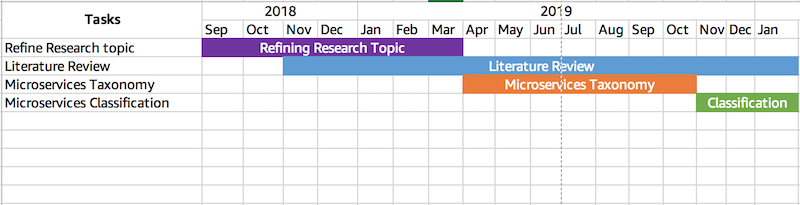
\includegraphics{projectplan.png}
\caption{Year One Schedule}
\end{figure}

\section{Why are the research questions interesting?}


I believe the selected research and the questions that it aims to answer will help fill a knowledge gap that exists today with microservices. Having the ability to classify, discover and compose microservices would be valuable at industry level as it would reduce wasted efforts in trying to build microservices that already exist thereby reducing development time and costs. The outcome of this research may also lay the foundation for devising a set of standards for building microservices though outside the scope of this project it may be a good opportunity to further this research. Last but not least, these research questions are a very interesting challenge for me and will give me the opportunity to acquire significant knowledge in an area of interest namely microservices.


\section{How it will be done?}

Building ML models requires dataset that will serve as training data and an algorithm that will help identify common patterns in the dataset and make human-like decisions or make predictions. For this project the plan is to use existing codes for commonly used services such as authentication service or a payment service to train the model and design an algorithm based on NLP framework that will help make decision on which service to build/produce based on user defined requirements.


\begin{figure}[h!]
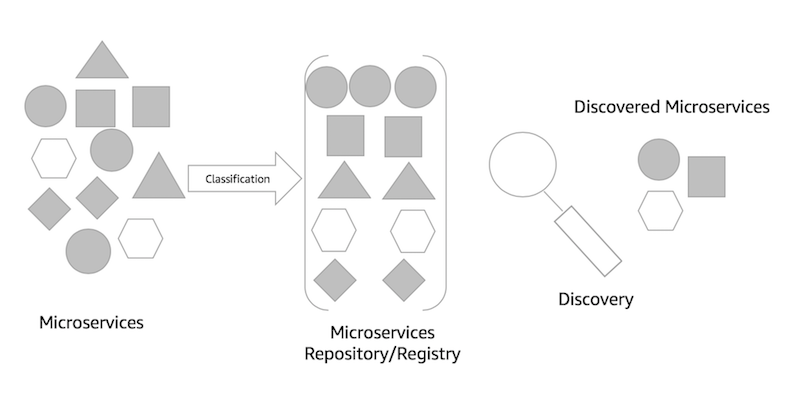
\includegraphics{discovery.png}
\caption{Microservices composition part one}
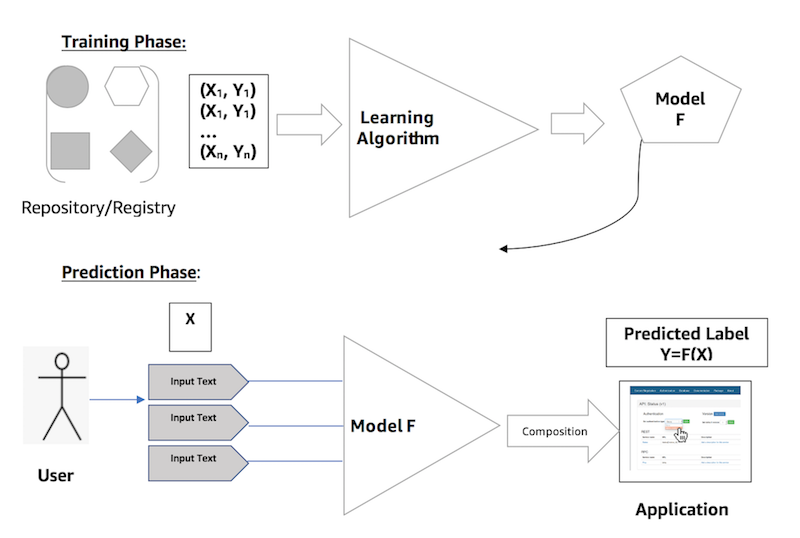
\includegraphics{mcsvcomposition.png}
\caption{Microservices composition part two}
\end{figure}

\pagebreak

\noindent As per the Figure 2 above, the training phase consists in using a set of frequently used microservices as dataset and design an algorithm that would identify with maximum precision possible microservices and produce a model (Model F) which basically enables microservices to respond to particular user’s inputs in plain English. 
\\
\\
\noindent In the prediction phase, a user enters his requirements for a particular microservice say an authentication service or a payment service, the model analyses the user inputs and triggers the discovery of relevant microservices and their composition into an application that is ready for use or require further customization by the user.


\section{Project work packages}

The project will be broken down into the following work packages:

\begin{enumerate}

\item \textbf{Classification}

The classification process will help with identification and grouping of microservices based on common properties. This will requires identifying the right semantics and producing a taxonomy to enable the classification process. 


\item \textbf{Repository and Registry}


In order to enable the discovery of microservices there would need to be stored into some type of repository with their attributes saved into some form of registry that the discovery engine can query to be able to retrieve microservices that meet the query criteria which in turn would depend on users ‘inputs. 


\item \textbf{Discovery module}


The discovery module as its name implies will serve the purpose of discovering microservices prior to their composition into the desired application taking place. The discovered microservices will be persisted into a buffer or temporary storage before being processed 


\item \textbf{User input module}


In order for user to obtain a specific functionality powered by a specific service or set services, he or she will be required to provide a number of specifications in plain in English as input. This process may be guided that is a user is restricted to specific type of inputs (e.g. an input form with specified attributes that need to be filled or menu selections), or completely open meaning user have the freedom to type any text they want to express their requirements and the model will interpret their inputs to produce the needed functionality in the form of coordinated microservices. The decision to use a guided or open approach for user inputs will depend on the complexity and the feasibility of one over the other within the scope of this project which means that one approach may constitute an opportunity for further research.


\item \textbf{Algorithm}


In order to identify pattern and learn from existing program/code and to translate users’ inputs into corresponding services one or more algorithms will be required which is basically a mathematical function that helps map an input to a desired output. Natural language processing (NLP) technologies in the way they work have a lot of similarities in terms of the problem this project is trying to solve so existing algorithms such as Naïve Bayes classifier, Probabilistic Context Free Grammar (PCFG) or Hidden Markov Model (HMM) to name but a few may be used or if necessary a completely new algorithm may be produced.


\item \textbf{Training data}


One of key steps in Machine and deep learning projects is to train the machine to be able to make predictions or human like decisions based on existing data. It is therefore vital that the data used to trained the machine be of very good quality. This work package will aim to do just that through data engineering steps that produce refined and good quality.


\item \textbf{Service repository framework}


A service repository framework is basically a repository that stores all the services that will represent the engine behind any business functionality requested by a user through the input module. It may use a Service Oriented Architecture approach that is provider-subscriber model where the user through their inputs will act as consumer requesting a service which will be provisioned by a service provider stored in some form of registry within the framework.


\item \textbf{Learning}


This phase consists in training the machine so that it can identify specific patterns from the training data. For this project the goal will be to identify the different services from various input sources and be able to map them to users’ inputs such that when a user enters his requirements for a specific functionality, the machine triggers the corresponding service or combination of services to produce the desired functionality.


\item \textbf{Prediction or Composition}


This work package is basically a model that will be tested again real data as opposed to the learning phase where training data will be used. Basically, once the training phase is complete we should end up with a model which can be used for processing users’ inputs and generating the desired functionalities by triggering the composition of relevant microservices. This process is depicted in Figure 3 above.


\item \textbf{Validation}


The validation phase will be all about comparing a functionality produced by the model to a similar functionality manually built or provided in a Software-as-a-Service (SaaS) model. This phase will help establish the viability of the model and what are the potential unique benefits it would offer to users in comparison to existing solutions available to them.

\end{enumerate}

\end{document}